
\documentclass{ppgeesa}

%%%%%%%%%%%%%%%%%%%%%%%%%%%%%%%%%%%%%%%%%%%%%%%%%%%%%%%%%%%%%%%%%%%%%%%%%%%%%%%%%%%%%%%%%%%%%%%%%%%%%%%%%%%%%%%%%

\usepackage[latin1]{inputenc}
\usepackage{graphicx}
\usepackage{hyperref}
\usepackage{tikz}
\usepackage{amsmath}
\usepackage{listings}

\lstset{ %
language=Matlab,                % choose the language of the code
basicstyle=\footnotesize,       % the size of the fonts that are used for the code
numbers=none,                   % where to put the line-numbers
numberstyle=\footnotesize,      % the size of the fonts that are used for the line-numbers
stepnumber=2,                   % the step between two line-numbers. If it's 1 each line 
                                % will be numbered
numbersep=5pt,                  % how far the line-numbers are from the code
backgroundcolor=\color{white},  % choose the background color. You must add \usepackage{color}
showspaces=false,               % show spaces adding particular underscores
showstringspaces=false,         % underline spaces within strings
showtabs=false,                 % show tabs within strings adding particular underscores
frame=false,	                % adds a frame around the code
tabsize=2,		                % sets default tabsize to 2 spaces
captionpos=b,                   % sets the caption-position to bottom
breaklines=true,                % sets automatic line breaking
breakatwhitespace=true,         % sets if automatic breaks should only happen at whitespace
title=\lstname,                 % show the filename of files included with \lstinputlisting;
                                % also try caption instead of title
escapeinside={\%*}{*)}         % if you want to add a comment within your code
%morekeywords={*,...}            % if you want to add more keywords to the set
}
\lstset{caption=Descriptive Caption Text,label=DescriptiveLabel}

\hypersetup{
	colorlinks,
	debug=true,
	linkcolor=black,  %%% cor do tableofcontents, \ref, \footnote, etc
	citecolor=red,  %%% cor do \cite
	urlcolor=blue,   %%% cor do \url e \href
	bookmarksopen=true,
	pdftitle={Modelagem e identifica��o de sistemas},
	pdfauthor={Tassiano Neuhaus},
	pdfsubject={M�todos param�tricos de identifica��o},
	pdfkeywords={Identifica��o de sistemas}
	%pdfpagemode=FullScreen
}

%%%%%%%%%%%%%%%%%%%%%%%%%%%%%%%%%%%%%%%%%%%%%%%%%%%%%%%%%%%%%%%%%%%%%%%%%%%%%%%%%%%%%%%%%%%%%%%%%%%%%%%%%%%%%%%%%


\begin{document}

\title{M�todos param�tricos de identifica��o de sistemas - Trabalho 4}

\author{Tassiano Neuhaus\\
{\small Universidade Federal do Rio Grande do Sul - Departamento de Engenharia El�trica\\Av. Osvaldo Aranha, 103 - Bairro Bom Fim CEP: 90035-190 - Porto Alegre - RS - Brasil}\\
}%\thanks{Tassiano Neuhaus, tassianors@gmail.com, tel +55-51-91760154}}

\maketitle
\thispagestyle{empty}\pagestyle{empty}

\begin{abstract}
Este trabalho tem o objetivo de demonstrar tr�s diferentes m�todos para estimativa do 
valor da resist�ncia de um resistor, baseado nas diversas medidas efetuadas sobre o mesmo, sendo que
estas medidas est�o sujeitas a incertezas de diversas fontes.

Ser� apresentado um algoritmo para identifica��o de par�metros para sistemas baseados no 
crit�rio de minimiza��o dos m�nimos quadrados. Ser� feio comparativos do m�todo para diferentes 
sinais de entrada e diferentes amplitudes de perturba��es sobre o sinal.
\end{abstract}

\begin{IEEEkeywords}
Identifica��o de sistemas lineares, m�todos param�tricos.
\end{IEEEkeywords}

%%===============================================================================
\section{Introdu��o}

Neste trabalho ser� apresentado o projeto de controladores denominados Robustos. Para 
tanto ser� apresentado o conceito de um controlador Robusto. A fim de modelar um
sistema sujeito a incertezas ser� apresentado alguns m�todos para que sua modelagem
matem�tica seja poss�vel. 

Para tornar o estudo mais claro ser� utilizado um sistema f�sico onde estar� sujeito a
perturba��es e/ou incertezas. Sobre este sistema ser� feito a modelagem seguindo cada um
dos processos e com estes modelos ser� efetuado uma simula��o. 

Esta simula��o ser� baseada no projeto de uma realimenta��o de estados com o intuito de
satisfazer a minimiza��o da norma $H2$ e $H_{\infty}$.

O sistema utilizado � apresentado no sistema de equa��es de estado descrito em (\ref{eq:intro_sis}).

\begin{equation}
\begin{matrix}
A=\begin{bmatrix}
0 & 1\\ 
-ba &a+b 
\end{bmatrix} &
B=\begin{bmatrix}
0\\ 
k
\end{bmatrix} 
\end{matrix}
\label{eq:intro_sis}
\end{equation}

Este sistema possui a fun��o de transfer�ncia apresentado em (\ref{eq:intro_transf}).

\begin{equation}
G(s)=\frac{k}{(s-a)(s-b)}
\label{eq:intro_transf}
\end{equation}

Os par�metros $a, b, k$ est�o sujeitos as varia��es apresentadas em (\ref{eq:intro_limit}).

\begin{equation}
\begin{matrix}
b= & -0.012725 & \\ 
k= & [k_1 \; k_2] =& [-0.4649.10^{-4} \; -0.7449.10^{-4}]\\ 
a= & [a_1 \; a_2] =& [-0.25 \; -2]
\end{matrix}
\label{eq:intro_limit}
\end{equation}


\section{Quest�o 1}
\label{sec:q1}
%===============================================================================

Quest�o: verificar de o LSE (estimador de m�nimos quadrados) produz estimativas 
n�o polarizadas no caso de estrituras do tipo ARX ARMAX e OE.

Genericamente, modelos utilizados para identifica��o de sistemas podem ser representados
pela equa��o (\ref{eq:q1_model}).

\begin{equation}
A(z, \theta)Y(t)=\frac{B(z, \theta)}{F(z, \theta)}U(t)+\frac{C(z, \theta)}{D(z, \theta)}e(t)
\label{eq:q1_model}
\end{equation}

Onde:

\begin{equation}
\begin{matrix}
A(z, \theta)=1+a_1 Z^{-1}+a_2 Z^{-2}+\cdots +a_{na} Z^{-na}\\
B(z, \theta)=b_1 Z^{-1}+b_2 Z^{-2}+\cdots +b_{nb} Z^{-nb}\\ 
C(z, \theta)=1+c_1 Z^{-1}+c_2 Z^{-2}+\cdots +c_{nc} Z^{-nc}\\ 
D(z, \theta)=1+d_1 Z^{-1}+d_2 Z^{-2}+\cdots +d_{na} Z^{-nd}\\ 
F(z, \theta)=1+f_1 Z^{-1}+f_2 Z^{-2}+\cdots +f_{nf} Z^{-nf} 
\end{matrix}
\nonumber
\end{equation}

Baseado nestas informa��es existem modelos onde apenas alguns destes polin�mios s�o 
diferentes de 1. Na Tabela (\ref{tab:model}) s�o apresentados alguns destes modelos
mais comumente utilizados.

\begin{table}[htbp]
  \begin{center}
	\caption{Modelos comumente utilizados para identifica��o de sistemas}
	\label{tab:model}
	\begin{small}
	  \begin{tabular}{rc}
		\hline
		Modelo & Polin�mios diferentes de 1 \\
		\hline
		FIR	& B \\
		ARX	& A B \\
		ARMAX & A B C \\
		ARMA & A C \\
		ARARMAX & A B C D \\
		OE & B F \\
		BJ & B F C D \\
		\hline
	  \end{tabular}
	\end{small}
  \end{center}
\end{table}


\subsection{ARX}
\label{sec:q1_arx}
%===============================================================================

A partir de (\ref{eq:q1_model}) tem-se que o modelo ARX fica (\ref{eq:q1_model_arx}).

\begin{equation}
A(z, \theta)Y(t)=B(z, \theta)U(t)+e(t)
\label{eq:q1_model_arx}
\end{equation}

A equa��o (\ref{eq:q1_model_arx}) pode ser reescrita :

\begin{equation}
\begin{matrix}
Y(t)=b_1 Z^{-1}U(t)+b_2 Z^{-2}U(t)+\cdots +b_{nb} Z^{-nb}U(t)\\
	 -a_1 Z^{-1}Y(t)-b_2 Z^{-2}Y(t)-\cdots -a_{na} Z^{-na}Y(t) + e(t)
\end{matrix}
\nonumber
\end{equation}

O que pode ser escrito como em (\ref{eq:q1_yt}).

\begin{equation}
Y(t)=\varphi ' \theta +e(t)
\label{eq:q1_yt}
\end{equation}

Onde:

\begin{equation}
\begin{matrix}
\theta = \begin{bmatrix}
a_1\\ 
\vdots \\ 
a_{na}\\ 
b_1\\ 
\vdots \\ 
b_{nb}
\end{bmatrix}
 & 
\varphi (t)=\begin{bmatrix}
y(t-1)\\ 
\vdots \\ 
y(t-na)\\ 
u(t-1)\\ 
\vdots \\ 
u(t-nb)
\end{bmatrix}
\\ 
& \\
\Phi = \begin{bmatrix}
\varphi '(1)\\ 
\varphi '(2)\\ 
\vdots\\ 
\varphi '(N)
\end{bmatrix} & 
\end{matrix}
\nonumber
\end{equation}

Pode -se ent�o encontrar a estimativa de $\theta$, ou seja $\hat{\theta}$.

\begin{equation}
\begin{matrix}
\hat{\theta}=(\Phi' \Phi)^{-1}(\Phi'(\Phi \theta_0+e))=\theta_0+(\Phi' \Phi)^{-1}\Phi'e\\ 
E\{ \hat{\theta} \}=\theta_0+(\Phi' \Phi)^{-1}\Phi'E\{ e(t)\}
\end{matrix}
\nonumber
\end{equation}

Mas como $E\{ e(t)\}=0$, pois o ruido possui m�dia zero. A estimativa de $\hat{\theta}$ � 
o pr�prio $\theta$.

De forma semelhante pode-se escrever:

\begin{equation}
\begin{matrix}
E\{(\hat{\theta}-\theta)(\hat{\theta}-\theta)' \}=E\{((\Phi'\Phi)^{-1}\Phi'e)((\Phi'\Phi)^{-1}\Phi'e)' \}
\\
=(\Phi'\Phi)^{-1}\Phi' E\{ e\; e'\}\Phi(\Phi'\Phi)^{-1}
\\ 
=E\{(\hat{\theta}-\theta)(\hat{\theta}-\theta)' \}=conv(\hat{\theta})=\lambda^2(\Phi'\Phi)^{-1}\\
pois : E\{ e\; e'\} = \lambda^2 I
\end{matrix}
\nonumber
\end{equation}

J� que a convolu��o da estimativa $\hat{\theta}$ corresponde ao valor encontrado, o
erro de polariza��o para o sistema ARX � igual a zero.


\subsection{ARMAX}
\label{sec:q1_armax}
%===============================================================================

A partir de (\ref{eq:q1_model}) tem-se que o modelo ARMAX fica (\ref{eq:q1_model_armax}).

\begin{equation}
A(z)Y(t)=B(z, \theta)U(t)+C(z, \theta)e(t)
\label{eq:q1_model_armax}
\end{equation}

A equa��o (\ref{eq:q1_model_armax}) pode ser reescrita :

\begin{equation}
\begin{matrix}
Y(t)=b_1 Z^{-1}U(t)+b_2 Z^{-2}U(t)+\cdots +b_{nb} Z^{-nb}U(t)\\
	 -a_1 Z^{-1}Y(t)-b_2 Z^{-2}Y(t)-\cdots -a_{na} Z^{-na}Y(t) + e(t)\\
	+c_1 Z^{-1}e(t)+c_2 Z^{-2}e(t)+\cdots +c_{nc} Z^{-nc}e(t)
\end{matrix}
\nonumber
\end{equation}

O que pode ser escrito como em (\ref{eq:q1_yt}). Onde:

\begin{equation}
\begin{matrix}
\theta = \begin{bmatrix}
a_1\\ 
\vdots \\ 
a_{na}\\ 
b_1\\ 
\vdots \\ 
b_{nb} \\
c_1\\ 
\vdots \\ 
c_{nc}
\end{bmatrix}
 & 
\varphi (t)=\begin{bmatrix}
y(t-1)\\ 
\vdots \\ 
y(t-na)\\ 
u(t-1)\\ 
\vdots \\ 
u(t-nb)\\
e(t-1)\\ 
\vdots \\ 
e(t-nb)
\end{bmatrix}
\\ 
& \\
\Phi = \begin{bmatrix}
\varphi '(1)\\ 
\varphi '(2)\\ 
\vdots\\ 
\varphi '(N)
\end{bmatrix} & 
\end{matrix}
\nonumber
\end{equation}

O sistema � apresentado na forma para que seja aplicado o crit�rio dos m�nimos quadrados
mas existem valores na matriz $\varphi(t)$ que n�o s�o mensur�veis ($e(t-1) ...$ ) o que 
torna o modelo n�o aplic�vel para este m�todo de minimiza��o. Desta forma se o m�todo 
for aplicado, teremos erro de polariza��o no resultado obtido.



\section{Quest�o 2}
\label{sec:q2}
%===============================================================================

Quest�o: Seja o sistema ARX (\ref{eq:q2arx}):

\begin{equation}
G_o(z)=\frac{2}{z-0.8}
\;\;
H_o(z)=\frac{z}{z-0.8}
\label{eq:q2arx}
\end{equation}

E com ruido branco com $ \lambda ^2 =0.1$.

\begin{itemize}
	\item Realize uma simula��o aplicando na entrada um ruido branco com $\lambda ^2=1$.
	\item Plote 100 estimativas de $\hat{\theta}$, a elipse de 95\% de confian�a e
	verifique o valor m�dio obtido e avalie a polariza��o da estimativa.
	\item Repita o item anterior com $H(z)=1$.
\end{itemize}

\subsection{Item 1 e 2}
%===============================================================================

Para realiza��o desta simula��o foi utilizado o script apresentado no Anexo 1.

Utilizando um ruido branco como entrada, com m�dia zero, e $\lambda ^2 = 1$, obt�m-se 
os resultados apresentados na Figura (\ref{fig:q2_noise}).

\begin{figure}[htbp]
	\center
	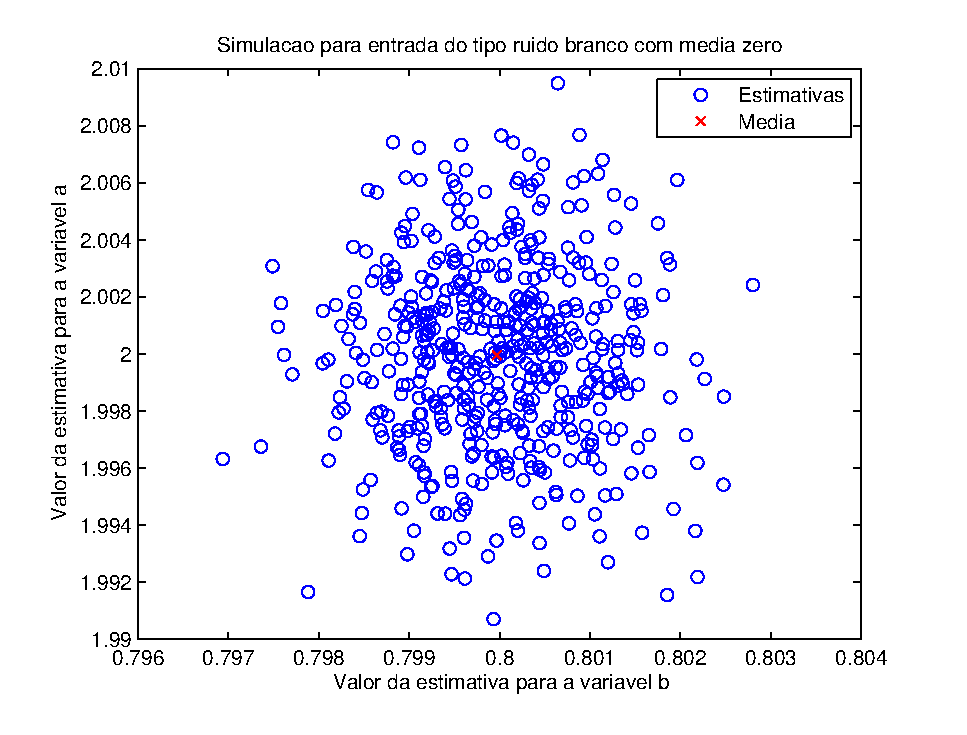
\includegraphics[width=0.98\columnwidth]{figures/q2_noise.eps}
	\caption{Entrada aleat�ria aplicada no processo para a identifica��o do sistema.}
	\label{fig:q2_noise}
\end{figure}

Observa-se que as estimativas em m�dia chegam relativamente pr�ximas ao valor real (a=2, b=0.8).
Desta forma conclui-se que n�o h� erro de polariza��o. Quando o ruido inserido n�o possui m�dia
zero, h� a observa��o de erro de polariza��o, como � apresentado na Figura (\ref{fig:q2_noise_pol}).

\begin{figure}[htbp]
	\center
	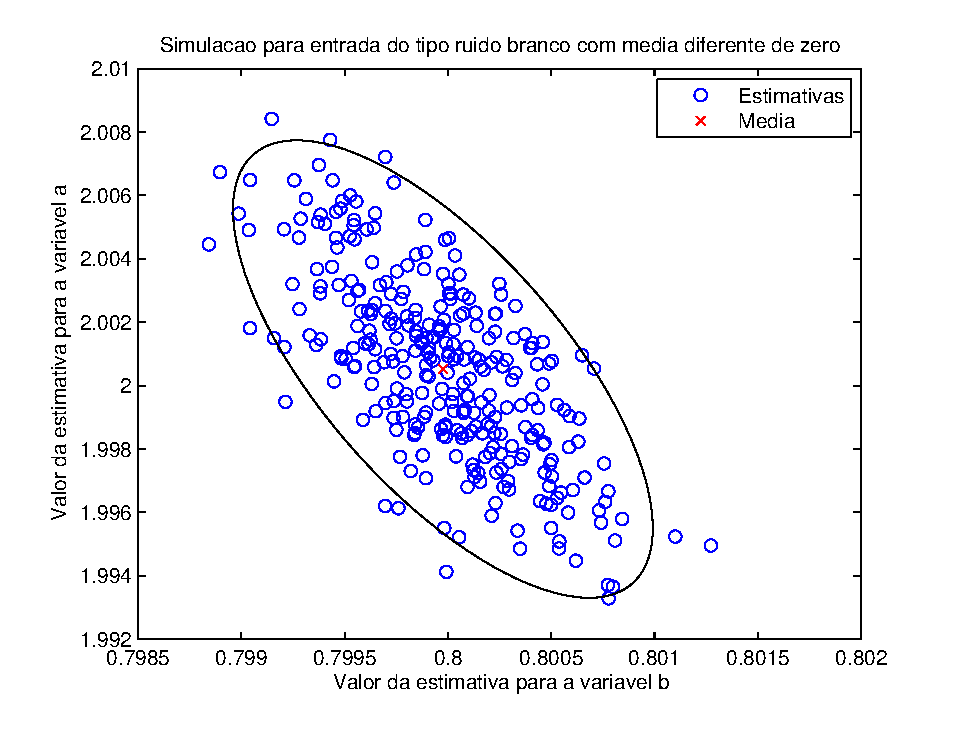
\includegraphics[width=0.98\columnwidth]{figures/q2_noise_pol.eps}
	\caption{Entrada aleat�ria aplicada no processo para a identifica��o do sistema. M�dia diferente de zero.}
	\label{fig:q2_noise}
\end{figure}

Neste caso, os valores m�dios encontrados foram b=0.8129 e a=2.003 e no caso onde a m�dia � zero, 
os valore estimados m�dios foram de a=1.9999 e b=0.8000.

\subsection{Item 3}
%===============================================================================

Na figura (\ref{fig:q2_noise_h1}) observa-se a simula��o para o mesmo sistema do item anterior,
mas com o ruido branco sujeito a fun��o de transfer�ncia $H(z) = 1$. Observa-se que a acuracidade
da m�dia dos pontos n�o � a mesma que quando a fun��o de transfer�ncia $H(z)$ � como em (\ref{eq:q2arx}).

\begin{figure}[htbp]
	\center
	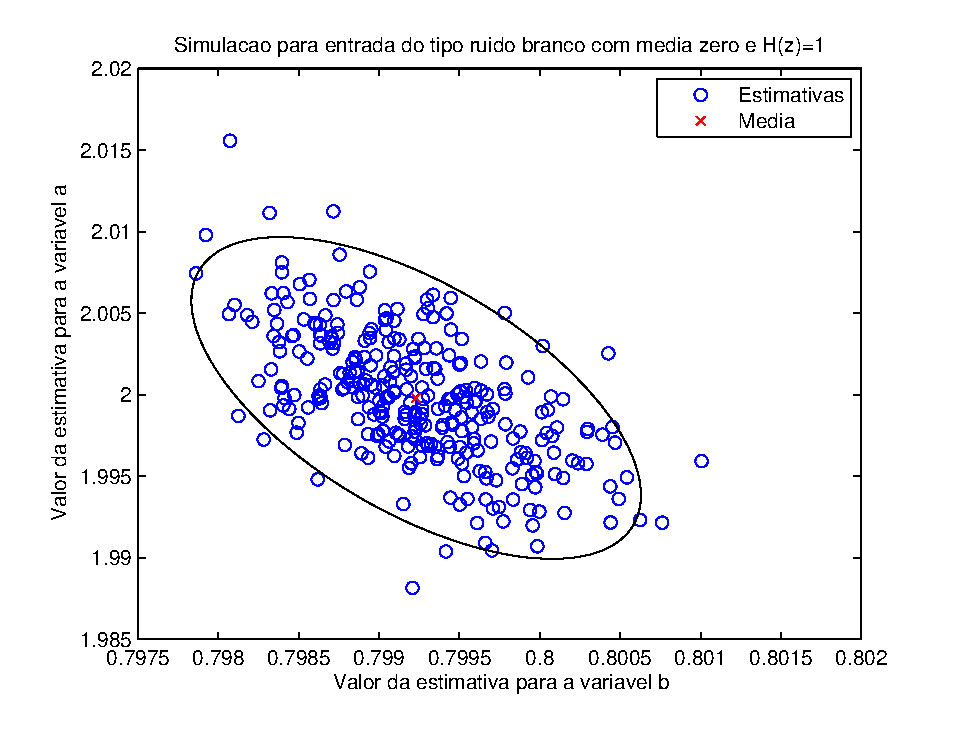
\includegraphics[width=0.98\columnwidth]{figures/q2_noise_h1.eps}
	\caption{Entrada aleat�ria aplicada no processo para a identifica��o do sistema. Ruido sujeito a
	$H(z)=1$.}
	\label{fig:q2_noise_h1}
\end{figure}

Outro ponto para destacar � que a elipse que para $H(z)$ como apresentado em (\ref{eq:q2arx}) era 
pr�xima � um circulo, neste exerc�cio com $H(z)=1$ � mais 'achatada', demonstrando que a confiabilidade
das estimativas n�o � mais sim�trica para as duas vari�veis em quest�o.



%%===============================================================================
\section{Conclus�es}
\label{sec:concl}
%===============================================================================

Neste trabalho foram apresentados dois m�todos para identifica��o de sistemas lineares,
ambos os m�todos se encontram na categoria de m�todos param�tricos de identifica��o, que 
de forma simplificada, tentam estimar os par�metros de uma fun��o de transfer�ncia que
represente o sistema f�sico em quest�o. Os m�todos utilizados foram o dos m�nimos quadrados
e das vari�veis instrumentais.

O sistema f�sico utilizado foi o controle de posi��o de um motor DC, e os dados coletados
para a identifica��o foram gerados a partir da aplica��o de sinais de refer�ncia tais como
rampas, senoides e ondas quadradas. Para cada um destes conjuntos foi obtido uma estimativa
dos par�metros do modelo utilizado.

Para efetuar a estimativa do sistema f�sico em quest�o, foi necess�rio determinar um modelo,
este foi determinado baseado no conhecimento das caracter�sticas do sistema e algumas simplifica��es 
foram efetuadas, a fim de tornar o modelo matem�tico o mais simples poss�vel, mas que ainda 
consiga descrever o sistema dentro de uma margem aceit�vel de precis�o.

O m�todo dos m�nimos quadrados (\ref{sec:mmq}) obteve resultados para a estimativa dos par�metros
que podem ser encontrados na Tabela (\ref{tab:mmq_results}). Houveram pequenas diverg�ncias nos 
par�metros entre um conjunto de dados e outro, o que n�o � desej�vel, isso pode ser devido a
imprecis�es do modelo utilizado, (pode ser devido as simplifica��es do modelo, ou de din�micas n�o
levadas em considera��o).

O m�todo das vari�veis instrumentais (\ref{sec:iv}) obteve resultados semelhantes ao m�todo 
dos m�nimos quadrados, mas com valores mais pr�ximos nos diferentes grupos de medidas. Os 
resultados para este m�todo foram apresentados na Tabela (\ref{tab:iv_results}).

De forma geral este trabalho abordou e demonstrou como � o procedimento e no que se baseiam 
dois m�todos de identifica��o de sistemas lineares sujeitos a incertezas, perturba��es e 
ru�dos. N�o � o objetivo deste trabalho detalhar esmiu�ar a matem�tica destes m�todos e
sim apresentar um exemplo pr�tico, e demonstrar sua utilidade.

A aplicabilidade deste t�pico de engenharia � de uma aplicabilidade imensa, sendo muito importante 
nas mais diversas �reas a correta identifica��o de sistemas para que, a partir do conhecimento 
matem�tico de sua din�mica, possa se agir sobre este sistema, a fim de obter os resultados desejados
de forma eficiente e com propriedade sobre as a��es tomadas, uma vez que o sistema identificado
� identificado e sabe-se o qu�o boa esta aproxima��o do sistema real pode ser.

%===============================================================================
\appendix
%===============================================================================
\chapter{1 - Script para Simula��o do MQ para o modelo ARX} 
\label{appendix_mmq}
\lstset{caption=M�todo dos m�nimos quadrados,label=DescriptiveLabel}
\lstinputlisting{matlab_files/simul.m}

%===============================================================================
\chapter{2 - Script para Simula��o do m�todo das vari�veis instrumentais} 
\label{appendix_iv}
\lstset{caption=M�todo das vari�veis instrumentais,label=DescriptiveLabel}
\lstinputlisting{matlab_files/simul_iv.m}

%===============================================================================



\bibliographystyle{IEEEtran}
\bibliography{biblio}

\end{document}
